%
% spielb.tex -- slide template
%
% (c) 2021 Prof Dr Andreas Müller, OST Ostschweizer Fachhochschule
%
\bgroup
\begin{frame}[t]
\setlength{\abovedisplayskip}{5pt}
\setlength{\belowdisplayskip}{5pt}
\frametitle{Modifiziertes Spiel $\tilde{B}$}
\vspace{-20pt}
\begin{columns}[t,onlytextwidth]
\begin{column}{0.48\textwidth}
\begin{block}{Definition}
Gewinn $\pm 1$, Wahrscheinlichkeit abhängig vom 3er-Rest des
aktuellen Kapitals $K$:
\begin{center}
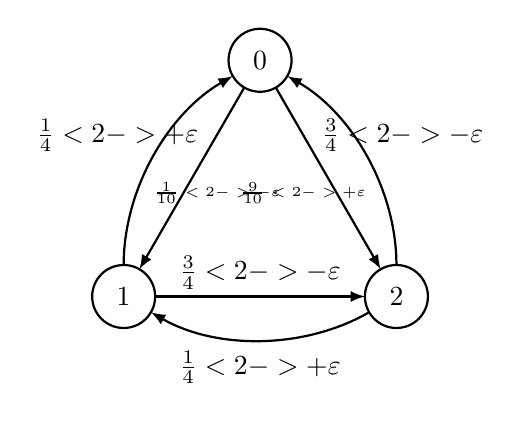
\begin{tikzpicture}[>=latex,thick]
\coordinate (A0) at (90:2);
\coordinate (A1) at (210:2);
\coordinate (A2) at (330:2);

\node at (A0) {$0$};
\node at (A1) {$1$};
\node at (A2) {$2$};

\draw (A0) circle[radius=0.4];
\draw (A1) circle[radius=0.4];
\draw (A2) circle[radius=0.4];

\draw[->,shorten >= 0.4cm,shorten <= 0.4cm] (A0) -- (A1);
\draw[->,shorten >= 0.4cm,shorten <= 0.4cm] (A0) -- (A2);
\draw[->,shorten >= 0.4cm,shorten <= 0.4cm] (A1) -- (A2);

\draw[->,shorten >= 0.4cm,shorten <= 0.4cm] (A1) to[out=90,in=-150] (A0);
\draw[->,shorten >= 0.4cm,shorten <= 0.4cm] (A2) to[out=90,in=-30] (A0);
\draw[->,shorten >= 0.4cm,shorten <= 0.4cm] (A2) to[out=-150,in=-30] (A1);

\def\R{1.9}
\def\r{0.7}

\node at (30:{0.9*\r}) {\tiny $\frac{9}{10}\uncover<2->{+\varepsilon}$};
\node at (150:{0.9*\r}) {\tiny $\frac1{10}\uncover<2->{-\varepsilon}$};
\node at (270:\r) {$\frac34\uncover<2->{-\varepsilon}$};

\node at (30:{1.1*\R}) {$\frac{3}{4}\uncover<2->{-\varepsilon}$};
\node at (150:{1.1*\R}) {$\frac1{4}\uncover<2->{+\varepsilon}$};
\node at (270:\R) {$\frac14\uncover<2->{+\varepsilon}$};

\end{tikzpicture}
\end{center}
\end{block}
\end{column}
\begin{column}{0.48\textwidth}
\begin{block}{Markov-Kette $\tilde{Y}$}
Übergangsmatrix
\[
\tilde{B}=
B\uncover<2->{+\varepsilon F}
\uncover<3->{=
B+\varepsilon\begin{pmatrix*}[r]
0&1&-1\\
-1&0&1\\
1&-1&0
\end{pmatrix*}}
\]
\vspace{-12pt}

\uncover<4->{%
Gewinnmatrix:
\[
G=\begin{pmatrix*}[r]
0&-1&1\\
1&0&-1\\
-1&1&0
\end{pmatrix*}
\]}
\end{block}
\vspace{-12pt}
\uncover<5->{%
\begin{block}{Gewinnerwartung}
\begin{align*}
\uncover<6->{E(\tilde{Y})
&=
U^t(G\odot \tilde{B})p}
\\
&\uncover<7->{=
E(Y) + \varepsilon U^t(G\odot F)p}
\uncover<8->{=
{\textstyle\frac1{15}}+2\varepsilon}
\\
\uncover<9->{
\text{rep.}
&=
-{\textstyle\frac{294}{169}}\varepsilon+O(\varepsilon^2)
\quad\text{Verlustspiel}
}
\end{align*}
\end{block}}
\end{column}
\end{columns}
\end{frame}
\egroup
